\newpage
\chapter{TINJAUAN PUSTAKA} \label{Bab II}

\section{Tinjauan Pustaka} \label{II.Tinjauan}
Penelitian disusun berdasarkan kajian terhadap beberapa penelitian terdahulu yang berkaitan dengan topik penanganan ketidakseimbangan data dalam klasifikasi. Kajian penelitian bertujuan untuk memahami pendekatan yang telah dikembangkan serta mengidentifikasi celah penelitian yang dapat dieksplorasi lebih lanjut.

Penelitian pertama dilakukan oleh Eroglu dan Pir (2024) yang mengusulkan metode hibrida bernama HOUM (\textit{Hybrid Oversampling and Undersampling Method}) \cite{Eroglu2024HOUM}. HOUM mengombinasikan Safe-Level SMOTE untuk \textit{oversampling} kelas minoritas dan SVM untuk \textit{undersampling} kelas mayoritas dalam proses iteratif. Pada setiap iterasi, SVM dilatih untuk membentuk \textit{decision boundary}, kemudian data mayoritas yang jauh dari \textit{hyperplane} dihapus dan data minoritas ditambahkan di posisi yang aman. Pengujian pada delapan dataset dari UCI \textit{Machine Learning Repository} menunjukkan bahwa HOUM mengungguli metode pembanding seperti SMOTE, SMOTEENN, SMOTETomek, W-SIMO, dan RusAda pada metrik G-mean dan ROC-AUC \cite{Eroglu2024HOUM}. Namun, penelitian tersebut hanya menggunakan konfigurasi \textit{default} pada komponen SVM tanpa mengkaji pengaruh variasi parameter $C$ dan jenis kernel.

Penelitian kedua berasal dari Taskiran \textit{et al.} (2025) yang mengevaluasi 31 teknik \textit{oversampling} untuk klasifikasi teks \cite{Taskiran2025Oversampling}. Evaluasi dilakukan pada dataset TREC dan Emotions menggunakan enam algoritma klasifikasi dengan representasi teks MiniLMv2. Teknik yang diuji meliputi SMOTE beserta 30 variannya, termasuk Borderline-SMOTE dan ADASYN. Hasil pengujian dengan metrik F1-Score dan \textit{Balanced Accuracy} menunjukkan bahwa tidak ada satu teknik \textit{oversampling} yang secara konsisten unggul di semua kondisi. Efektivitas teknik sangat bergantung pada karakteristik distribusi data dan algoritma klasifikasi yang digunakan \cite{Taskiran2025Oversampling}.

Penelitian ketiga merupakan karya Hou \textit{et al.} (2025) yang membandingkan delapan teknik \textit{resampling} untuk prediksi \textit{financial distress} menggunakan XGBoost \cite{Hou2025XGBoost}. Teknik yang diuji meliputi SMOTE, ADASYN, Borderline-SMOTE, Tomek Links, \textit{Random Under-Sampling}, SMOTE-Tomek, SMOTE-ENN, dan Bagging-SMOTE. Hasil eksperimen menunjukkan bahwa SMOTE mencapai F1-score tertinggi sebesar 0,73 dengan MCC 0,70, sedangkan Bagging-SMOTE memperoleh F1-score 0,72 dengan AUC 0,96. \textit{Random Under-Sampling} menghasilkan \textit{recall} tinggi (0,85) namun \textit{precision} rendah (0,46), sehingga kurang tepat untuk kasus yang memerlukan keseimbangan kedua metrik \cite{Hou2025XGBoost}. Temuan ini memperkuat argumen bahwa teknik \textit{undersampling} acak berpotensi menurunkan kualitas data pelatihan.

Penelitian keempat diambil dari Tariq \textit{et al.} (2023) yang menguji metode \textit{oversampling} pada dataset pendidikan bertipe \textit{multi-class} \cite{Tariq2023Oversampling}. Metode yang diuji meliputi SMOTE, ADASYN, Borderline-SMOTE, dan SMOTETomek yang dikombinasikan dengan sepuluh algoritma klasifikasi. Hasil pengujian menunjukkan bahwa kombinasi SMOTETomek dengan KNN mencapai akurasi tertinggi sebesar 83,7\%. Temuan ini mengindikasikan bahwa pendekatan hibrida yang menggabungkan \textit{oversampling} dengan pembersihan data memberikan hasil lebih baik dibandingkan \textit{oversampling} tunggal \cite{Tariq2023Oversampling}. Penelitian tersebut menunjukkan bahwa pemilihan algoritma klasifikasi turut memengaruhi efektivitas teknik \textit{oversampling} yang diterapkan.

Penelitian kelima dilakukan oleh Van FC \textit{et al.} (2024) yang menerapkan SMOTE dan \textit{random undersampling} pada klasifikasi sentimen media sosial menggunakan SVM \cite{VanFC2024Enhancing}. Dataset yang digunakan berasal dari platform Twitter terkait Pemilu 2024 dengan distribusi kelas yang tidak seimbang. Tiga variasi kernel SVM diuji, yaitu Linear, RBF, dan Polynomial. Hasil percobaan menunjukkan bahwa SMOTE mampu meningkatkan akurasi SVM hingga 91\%, khususnya pada kernel Polynomial yang menunjukkan peningkatan paling signifikan \cite{VanFC2024Enhancing}. Sebaliknya, teknik \textit{random undersampling} tidak memberikan peningkatan yang berarti pada seluruh variasi kernel yang diuji.

Berdasarkan tinjauan terhadap kelima penelitian pada Tabel \ref{tab:2.tinjauan}, dapat diidentifikasi bahwa teknik \textit{resampling} hibrida mampu meningkatkan performa klasifikasi pada data tidak seimbang. Namun demikian, terdapat celah penelitian yang belum dieksplorasi. Pertama, HOUM yang diusulkan oleh Eroglu dan Pir hanya menggunakan konfigurasi \textit{default} pada komponen SVM tanpa mengkaji pengaruh variasi parameter $C$ dan jenis kernel \cite{Eroglu2024HOUM}. Kedua, komponen \textit{oversampling} pada HOUM hanya menggunakan Safe-Level SMOTE tanpa membandingkannya dengan teknik adaptif seperti ADASYN. Oleh karena itu, penelitian ini mengisi celah tersebut melalui variasi parameter $C$ pada SVM (0,5; 1; 1,5; 2; 2,5; dan 3), perbandingan tiga jenis kernel (Linear, RBF, dan Polynomial), serta komparasi Safe-Level SMOTE dan ADASYN sebagai komponen \textit{oversampling} pada HOUM.


\section{Dasar Teori} \label{II.Teori}
Pada bagian ini dijelaskan konsep-konsep teoritis yang mendasari penelitian ini sebagai berikut. \par

\subsection{Klasifikasi} \label{II.klasifikasi}
Klasifikasi menjadi salah satu tugas utama dalam \textit{machine learning} yang bertujuan memetakan data masukan ke dalam kategori atau kelas yang telah ditentukan sebelumnya \cite{Sarker2021ML}. Model klasifikasi dibangun melalui proses pelatihan menggunakan dataset berlabel, dimana algoritma mempelajari hubungan antara fitur masukan dan kelas keluaran. Setelah proses pelatihan selesai, model yang dihasilkan dapat digunakan untuk memprediksi kelas dari data baru yang tidak terdapat dalam dataset pelatihan. Tahapan utama dalam klasifikasi meliputi prapemrosesan data, ekstraksi fitur, pemilihan algoritma, pelatihan model, serta validasi menggunakan data uji \cite{Sarker2021ML, Mohammed2020Resampling}. Kualitas hasil klasifikasi sangat dipengaruhi oleh representasi fitur yang digunakan dan kesesuaian algoritma terhadap karakteristik dataset.

Berdasarkan jumlah kelas keluaran, klasifikasi dibedakan menjadi dua jenis utama, yaitu klasifikasi \textit{binary} yang melibatkan dua kelas dan klasifikasi \textit{multi-class} yang melibatkan lebih dari dua kelas \cite{Sarker2021ML}. Klasifikasi \textit{binary} banyak diterapkan pada permasalahan seperti deteksi penipuan, diagnosis penyakit, dan deteksi intrusi jaringan yang memerlukan pemisahan antara kelas positif dan negatif \cite{He2009Imbalanced}. Klasifikasi \textit{multi-class} diterapkan pada pengenalan karakter tulisan tangan, analisis sentimen multi-kategori, dan klasifikasi citra \cite{Abdullah2021SVM}. Beberapa algoritma klasifikasi yang banyak digunakan meliputi \textit{Decision Tree}, \textit{K-Nearest Neighbors} (KNN), \textit{Naive Bayes}, \textit{Random Forest}, dan \textit{Support Vector Machine} (SVM) \cite{Cervantes2020SVM}. Pemilihan algoritma yang tepat menjadi faktor penting yang menentukan akurasi dan kemampuan generalisasi model klasifikasi \cite{Abdullah2021SVM}.


\subsection{Ketidakseimbangan Data (\textit{Class Imbalance})} \label{II.imbalanced}
He dan Garcia (2009) mendefinisikan \textit{imbalanced learning} sebagai permasalahan yang muncul ketika distribusi kelas dalam dataset pelatihan tidak seimbang, sehingga performa algoritma klasifikasi standar menjadi terganggu \cite{He2009Imbalanced}. Kelas dengan jumlah sampel lebih banyak disebut kelas mayoritas, sedangkan kelas dengan jumlah sampel lebih sedikit disebut kelas minoritas. Rasio ketidakseimbangan antar kelas dapat bervariasi dari 100:1, 1.000:1, hingga 10.000:1, dimana satu kelas secara signifikan mendominasi kelas lainnya \cite{He2009Imbalanced}. Kondisi ini banyak ditemui pada dataset dunia nyata seperti deteksi penipuan kartu kredit, diagnosis penyakit langka, deteksi intrusi jaringan, dan klasifikasi citra biomedis \cite{Krawczyk2016Imbalanced, Thabtah2020DataImbalance}. Semakin tinggi rasio ketidakseimbangan, semakin sulit bagi algoritma klasifikasi konvensional untuk mempelajari pola kelas minoritas secara efektif \cite{Haixiang2017Survey}. Ilustrasi distribusi data tidak seimbang ditunjukkan pada Gambar \ref{fig:2.imbalanced}.

\begin{figure}[H]
    \centering
    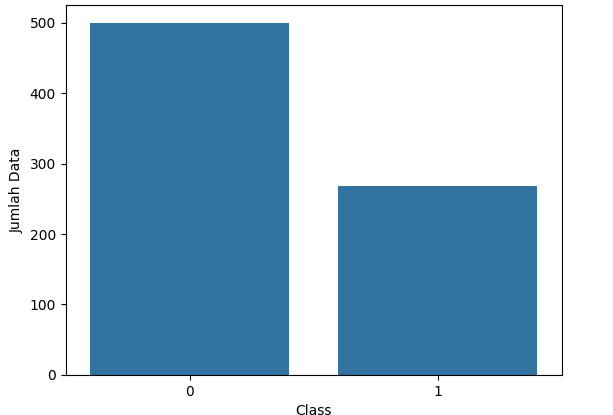
\includegraphics[width=0.6\textwidth]{figure/imbalanced.png}
    \caption{Ilustrasi Distribusi Data Tidak Seimbang}
    \label{fig:2.imbalanced}
\end{figure}

Algoritma klasifikasi standar pada umumnya dirancang untuk meminimalkan kesalahan klasifikasi secara keseluruhan tanpa memperhatikan distribusi kelas \cite{Chawla2002SMOTE}. Chawla \textit{et al.} (2002) menyatakan bahwa metrik akurasi tidak tepat digunakan pada data tidak seimbang karena strategi sederhana berupa prediksi seluruh data ke kelas mayoritas sudah dapat menghasilkan akurasi yang tinggi \cite{Chawla2002SMOTE}. He dan Garcia (2009) memberikan contoh pada dataset mammografi yang berisi 10.923 sampel negatif dan 260 sampel positif, dimana klasifier cenderung menghasilkan akurasi mendekati 100\% pada kelas mayoritas namun hanya 0-10\% pada kelas minoritas \cite{He2009Imbalanced}. Konsekuensi dari bias semacam ini dapat sangat merugikan pada domain seperti kedokteran, dimana kegagalan mendeteksi pasien sakit jauh lebih berbahaya daripada kesalahan diagnosis sebaliknya \cite{He2009Imbalanced}. Oleh karena itu, diperlukan metrik evaluasi yang lebih informatif seperti kurva ROC, \textit{precision-recall}, dan \textit{cost curves} untuk menilai performa model secara menyeluruh \cite{He2009Imbalanced, Fawcett2006ROC}.

Tingkat ketidakseimbangan pada suatu dataset dapat diukur menggunakan \textit{imbalance ratio} (IR), yaitu perbandingan antara jumlah sampel kelas mayoritas dengan jumlah sampel kelas minoritas sebagaimana ditunjukkan pada \ref{eq:2.ir}.

\begin{equationcaptioned}[eq:2.ir]{
    IR = \frac{N_{majority}}{N_{minority}}
}{
    Imbalance Ratio (IR)
}
\end{equationcaptioned}

Keterangan: \\
$N_{majority}$ = jumlah sampel kelas mayoritas \\
$N_{minority}$ = jumlah sampel kelas minoritas

He dan Garcia (2009) mengklasifikasikan pendekatan penanganan data tidak seimbang ke dalam empat kategori utama \cite{He2009Imbalanced}. Kategori pertama adalah metode \textit{sampling} yang memodifikasi distribusi dataset melalui teknik \textit{oversampling} atau \textit{undersampling} untuk menyeimbangkan representasi kelas. Kategori kedua adalah \textit{cost-sensitive learning} yang menetapkan biaya berbeda untuk kesalahan klasifikasi pada masing-masing kelas, sehingga kesalahan pada kelas minoritas mendapat penalti yang lebih besar \cite{He2009Imbalanced}. Kategori ketiga adalah metode berbasis kernel yang memodifikasi matriks kernel untuk mengakomodasi ketidakseimbangan distribusi data \cite{He2009Imbalanced}. Kategori keempat adalah \textit{active learning} yang secara selektif memilih sampel paling informatif untuk pelabelan guna mengurangi biaya komputasi pada dataset tidak seimbang yang besar \cite{He2009Imbalanced}.


\subsection{\textit{Oversampling}} \label{II.oversampling}
\textit{Oversampling} termasuk teknik penanganan data tidak seimbang pada level data yang bekerja dengan menambah jumlah sampel pada kelas minoritas hingga distribusi antar kelas menjadi lebih seimbang. Bunkhumpornpat \textit{et al.} (2009) menjelaskan bahwa teknik \textit{re-sampling} paling sederhana adalah \textit{random oversampling} yang menduplikasi sampel kelas minoritas secara acak hingga kedua kelas memiliki representasi yang setara \cite{Bunkhumpornpat2009SafeLevel}. Namun, teknik ini berpotensi menyebabkan \textit{overfitting} karena area keputusan yang dihasilkan menjadi lebih sempit dan spesifik akibat duplikasi data identik \cite{Bunkhumpornpat2009SafeLevel}. Untuk mengatasi keterbatasan tersebut, dikembangkan teknik \textit{oversampling} berbasis sintesis yang menghasilkan sampel baru melalui interpolasi antar data minoritas yang sudah ada \cite{Chawla2002SMOTE}. Kov\'{a}cs (2019) melakukan perbandingan empiris terhadap 85 teknik \textit{oversampling} minoritas pada 104 dataset dan menemukan bahwa teknik sintesis data secara signifikan mengungguli \textit{random oversampling} dalam berbagai skenario klasifikasi \cite{Kovacs2019Empirical, Kovacs2019SmoteVariants}. Ilustrasi teknik \textit{oversampling} ditunjukkan pada Gambar \ref{fig:2.oversampling}.

\begin{figure}[H]
    \centering
    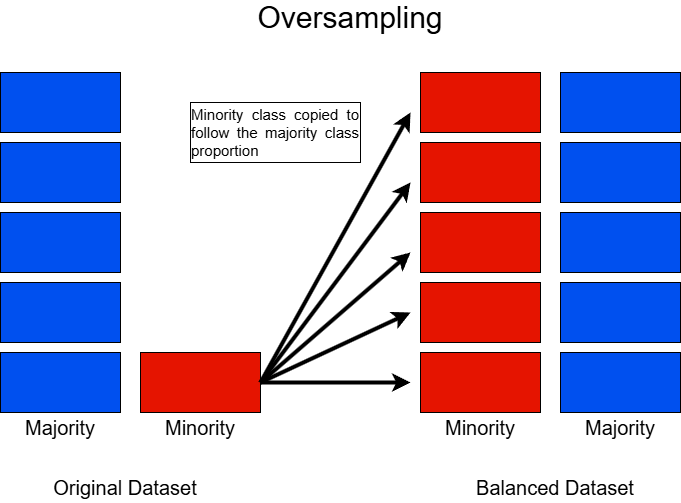
\includegraphics[width=0.8\textwidth]{figure/oversampling.png}
    \caption{Ilustrasi Teknik \textit{Oversampling}}
    \label{fig:2.oversampling}
\end{figure}

\subsubsection{SMOTE (\textit{Synthetic Minority Over-sampling Technique})} \label{II.smote}
Chawla \textit{et al.} (2002) mengusulkan SMOTE sebagai teknik \textit{oversampling} dengan pendekatan menghasilkan sampel sintetis kelas minoritas melalui interpolasi antar sampel yang sudah ada \cite{Chawla2002SMOTE}. Chawla \textit{et al.} menyatakan bahwa SMOTE bekerja dengan mengambil setiap sampel kelas minoritas, kemudian menghasilkan data sintetis di sepanjang segmen garis yang menghubungkan sampel tersebut dengan $k$ tetangga terdekatnya dari kelas yang sama \cite{Chawla2002SMOTE}. Pendekatan ini menghasilkan area keputusan yang lebih luas dan umum dibandingkan \textit{random oversampling} yang hanya menduplikasi data identik \cite{Chawla2002SMOTE}. Elreedy dan Atiya (2019) mencatat bahwa SMOTE telah menjadi salah satu teknik penanganan data tidak seimbang yang paling dominan dalam literatur dan menjadi fondasi bagi pengembangan lebih dari 85 varian \cite{Elreedy2023SMOTE, Kovacs2019SmoteVariants}. Proses pembentukan sampel sintetis secara matematis ditunjukkan pada \ref{eq:2.smote}.

\begin{equationcaptioned}[eq:2.smote]{
    x_{new} = x_i + \lambda \times (x_{nn} - x_i)
}{
    Pembentukan Sampel Sintetis SMOTE
}
\end{equationcaptioned}

Keterangan: \\
$x_{new}$ = sampel sintetis baru \\
$x_i$ = sampel kelas minoritas \\
$x_{nn}$ = tetangga terdekat yang dipilih \\
$\lambda$ = bilangan acak dalam rentang [0, 1]

Bunkhumpornpat \textit{et al.} (2009) mengidentifikasi bahwa SMOTE memiliki kelemahan berupa masalah \textit{overgeneralization}, yaitu SMOTE secara buta memperluas area kelas minoritas tanpa mempertimbangkan keberadaan kelas mayoritas di sekitarnya \cite{Bunkhumpornpat2009SafeLevel}. Strategi ini menjadi problematik pada distribusi kelas yang sangat timpang karena kelas minoritas tersebar sangat jarang di antara kelas mayoritas, sehingga peluang tercampurnya kedua kelas menjadi lebih besar \cite{Bunkhumpornpat2009SafeLevel}. Han \textit{et al.} (2005) mengamati bahwa sampel sintetis yang dihasilkan di area \textit{noise} atau di dalam wilayah kelas mayoritas dapat mengaburkan batas keputusan dan menurunkan performa klasifikasi \cite{Han2005BorderlineSMOTE}. Kelemahan-kelemahan ini mendorong pengembangan berbagai varian SMOTE seperti Borderline-SMOTE yang hanya melakukan interpolasi pada sampel di area perbatasan, Safe-Level SMOTE yang mempertimbangkan tingkat keamanan posisi interpolasi, dan ADASYN yang mendistribusikan sampel sintetis secara adaptif \cite{Han2005BorderlineSMOTE, Bunkhumpornpat2009SafeLevel, He2008ADASYN}. Tarawneh \textit{et al.} (2022) menambahkan bahwa sensitivitas SMOTE terhadap \textit{outlier} menjadi perhatian utama karena sampel minoritas yang merupakan \textit{outlier} tetap dijadikan basis interpolasi \cite{Tarawneh2022SMOTEFUNA}.

\subsubsection{Safe-Level SMOTE} \label{II.safelevel}
Bunkhumpornpat \textit{et al.} (2009) mengembangkan Safe-Level SMOTE dari SMOTE untuk mengatasi masalah pembentukan sampel sintetis di area yang tidak aman \cite{Bunkhumpornpat2009SafeLevel}. Konsep utama metode ini adalah memberikan setiap sampel kelas minoritas suatu nilai \textit{safe level} sebelum proses sintesis dilakukan. Bunkhumpornpat \textit{et al.} mendefinisikan \textit{safe level} sebagai jumlah tetangga terdekat yang berasal dari kelas minoritas yang sama \cite{Bunkhumpornpat2009SafeLevel}. Sampel dengan \textit{safe level} mendekati $k$ menandakan bahwa sampel tersebut berada di area yang aman dan didominasi oleh kelasnya sendiri. Sebaliknya, sampel dengan \textit{safe level} mendekati 0 mengindikasikan sampel yang mendekati \textit{noise} karena dikelilingi oleh kelas mayoritas \cite{Bunkhumpornpat2009SafeLevel}.

Penempatan sampel sintetis ditentukan oleh \textit{safe level ratio} antara sampel asli $p$ dan tetangga $n$ yang dihitung sebagai $sl_p / sl_n$ \cite{Bunkhumpornpat2009SafeLevel}. Bunkhumpornpat \textit{et al.} mendefinisikan lima kasus berdasarkan nilai rasio ini. Apabila rasio bernilai tak hingga dan \textit{safe level} keduanya nol, maka keduanya dianggap \textit{noise} dan sampel sintetis tidak dihasilkan. Apabila rasio bernilai tak hingga namun \textit{safe level} $p$ bukan nol, maka sampel sintetis dihasilkan dengan menduplikasi $p$ untuk menjauhi tetangga yang merupakan \textit{noise}. Apabila rasio bernilai 1, sampel sintetis ditempatkan di posisi acak sepanjang garis antara $p$ dan $n$ karena keduanya memiliki tingkat keamanan yang setara \cite{Bunkhumpornpat2009SafeLevel}. Apabila rasio lebih besar dari 1, sampel sintetis ditempatkan lebih dekat ke $p$ yang lebih aman, dan sebaliknya apabila rasio kurang dari 1, sampel ditempatkan lebih dekat ke $n$ \cite{Bunkhumpornpat2009SafeLevel}. Hasil eksperimen Bunkhumpornpat \textit{et al.} menunjukkan bahwa Safe-Level SMOTE menghasilkan akurasi yang lebih baik dibandingkan SMOTE dan Borderline-SMOTE pada berbagai dataset pengujian \cite{Bunkhumpornpat2009SafeLevel}.

\subsubsection{ADASYN (\textit{Adaptive Synthetic Sampling})} \label{II.adasyn}
He \textit{et al.} (2008) mengusulkan ADASYN sebagai teknik \textit{oversampling} adaptif dengan ide utama menggunakan distribusi berbobot untuk sampel kelas minoritas berdasarkan tingkat kesulitan dalam proses klasifikasi \cite{He2008ADASYN}. He \textit{et al.} menjelaskan bahwa ADASYN menghasilkan lebih banyak data sintetis untuk sampel kelas minoritas yang lebih sulit dipelajari dibandingkan sampel yang lebih mudah \cite{He2008ADASYN}. Pendekatan ini mempunyai dua tujuan: mengurangi bias yang ditimbulkan oleh ketidakseimbangan distribusi kelas, dan secara adaptif menggeser batas keputusan ke arah sampel yang sulit diklasifikasikan \cite{He2008ADASYN}. Tahap pertama ADASYN menghitung derajat ketidakseimbangan $d = m_s / m_l$ dan total sampel sintetis yang diperlukan $G = (m_l - m_s) \times \beta$, dimana $\beta \in [0,1]$ menentukan tingkat keseimbangan yang diinginkan \cite{He2008ADASYN}. Distribusi bobot yang menentukan jumlah sampel sintetis untuk setiap sampel kelas minoritas dihitung sebagaimana ditunjukkan pada \ref{eq:2.adasyn}.

\begin{equationcaptioned}[eq:2.adasyn]{
    \hat{r}_i = \frac{r_i}{\sum_{i=1}^{m_s} r_i}, \quad r_i = \frac{\Delta_i}{k}
}{
    Distribusi Bobot ADASYN
}
\end{equationcaptioned}

Keterangan: \\
$\hat{r}_i$ = bobot ternormalisasi sampel $x_i$ \\
$\Delta_i$ = jumlah tetangga dari kelas mayoritas \\
$k$ = jumlah tetangga terdekat \\
$m_s$ = total sampel kelas minoritas

Jumlah sampel sintetis untuk setiap $x_i$ dihitung menggunakan formula $g_i = \hat{r}_i \times G$, dimana $G$ menyatakan total sampel yang perlu ditambahkan agar distribusi kelas menjadi seimbang \cite{He2008ADASYN}. He \textit{et al.} menjelaskan bahwa $\hat{r}_i$ secara fisik menjadi pengukuran distribusi bobot untuk berbagai sampel kelas minoritas berdasarkan tingkat kesulitannya dalam proses pembelajaran \cite{He2008ADASYN}. Sampel dengan nilai $\hat{r}_i$ lebih tinggi berarti dikelilingi oleh lebih banyak tetangga kelas mayoritas sehingga lebih sulit diklasifikasikan dan memperoleh lebih banyak data sintetis \cite{He2008ADASYN}. Setiap sampel sintetis dibentuk melalui interpolasi $s_i = x_i + (x_{zi} - x_i) \times \lambda$ dengan $\lambda \in [0,1]$ dan $x_{zi}$ merupakan tetangga minoritas yang dipilih secara acak \cite{He2008ADASYN}. Namun, Elreedy dan Atiya (2019) mencatat bahwa ADASYN berpotensi menghasilkan data sintetis di area \textit{noise} apabila sampel minoritas yang menjadi acuan merupakan \textit{outlier} yang dikelilingi oleh kelas mayoritas \cite{Elreedy2023SMOTE}.


\subsection{\textit{Undersampling}} \label{II.undersampling}
\textit{Undersampling} termasuk teknik penanganan data tidak seimbang yang bekerja dengan mengurangi jumlah sampel pada kelas mayoritas hingga distribusi antar kelas menjadi lebih proporsional. Bunkhumpornpat \textit{et al.} (2009) menyatakan bahwa \textit{random undersampling} menghapus sampel kelas mayoritas secara acak hingga kedua kelas memiliki jumlah yang setara, namun teknik ini berpotensi menghilangkan informasi penting dari dataset \cite{Bunkhumpornpat2009SafeLevel}. Elreedy dan Atiya (2019) mencatat bahwa \textit{undersampling} bersifat berisiko karena informasi penting yang potensial dapat hilang dari proses penghapusan \cite{Elreedy2023SMOTE}. Untuk mengatasi risiko tersebut, dikembangkan teknik \textit{undersampling} yang lebih terstruktur berdasarkan aturan heuristik tertentu. Beberapa teknik yang banyak digunakan antara lain Tomek Links, \textit{Edited Nearest Neighbors} (ENN), \textit{condensed nearest neighbor rule}, dan \textit{one-sided selection} \cite{Elreedy2023SMOTE, Batista2004Balancing}. Ilustrasi teknik \textit{undersampling} ditunjukkan pada Gambar \ref{fig:2.undersampling}.

\begin{figure}[H]
    \centering
    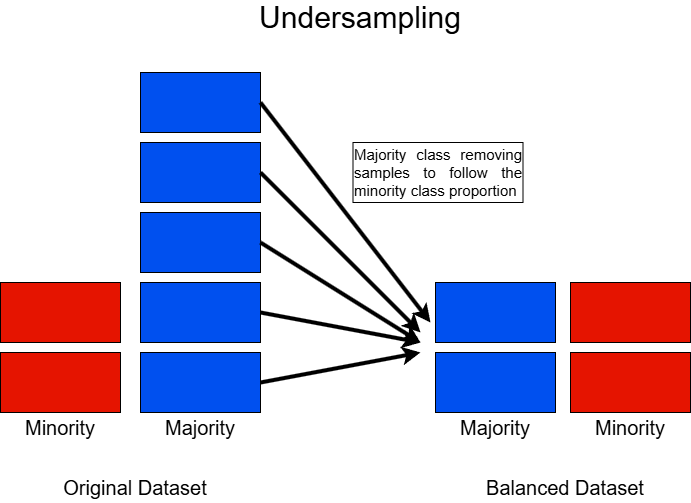
\includegraphics[width=0.8\textwidth]{figure/undersampling.png}
    \caption{Ilustrasi Teknik \textit{Undersampling}}
    \label{fig:2.undersampling}
\end{figure}


\subsection{Metode Hibrida (\textit{Hybrid Resampling})} \label{II.hybrid}
Metode hibrida menggabungkan teknik \textit{oversampling} dan \textit{undersampling} dalam satu kerangka kerja untuk menangani data tidak seimbang dengan memanfaatkan kelebihan keduanya secara bersamaan. He dan Garcia (2009) menjelaskan bahwa komunitas \textit{machine learning} menangani permasalahan ketidakseimbangan kelas melalui dua cara utama: memberikan biaya berbeda pada setiap sampel pelatihan, atau melakukan \textit{re-sampling} melalui \textit{oversampling} kelas minoritas dan/atau \textit{undersampling} kelas mayoritas \cite{He2009Imbalanced}. Chawla \textit{et al.} (2002) menunjukkan bahwa kombinasi \textit{oversampling} kelas minoritas menggunakan SMOTE dengan \textit{undersampling} kelas mayoritas menghasilkan performa klasifikasi yang lebih baik dalam ruang ROC dibandingkan penggunaan \textit{undersampling} tunggal \cite{Chawla2002SMOTE}. Penggabungan kedua teknik bertujuan menghasilkan dataset yang seimbang tanpa kehilangan informasi penting dari kelas mayoritas maupun menciptakan \textit{overfitting} pada kelas minoritas. Pendekatan ini telah terbukti efektif pada berbagai domain aplikasi.

Batista \textit{et al.} (2004) memperkenalkan dua kombinasi hibrida yang paling banyak dirujuk dalam literatur, yaitu SMOTETomek dan SMOTEENN \cite{Batista2004Balancing}. SMOTETomek mengombinasikan SMOTE untuk menambah sampel kelas minoritas dengan Tomek Links untuk menghapus pasangan sampel yang saling berdekatan dari kelas berbeda. SMOTEENN mengombinasikan SMOTE dengan \textit{Edited Nearest Neighbors} yang membersihkan sampel yang salah diklasifikasikan oleh tetangga terdekatnya. Batista \textit{et al.} menunjukkan melalui eksperimen pada 13 dataset bahwa SMOTETomek dan SMOTEENN secara konsisten menghasilkan performa yang lebih baik dibandingkan SMOTE atau \textit{random undersampling} secara terpisah \cite{Batista2004Balancing}. Temuan serupa dilaporkan oleh Hou \textit{et al.} (2025) pada domain prediksi \textit{financial distress} yang mengonfirmasi keunggulan pendekatan hibrida dibandingkan teknik tunggal \cite{Hou2025XGBoost}.


\subsection{HOUM (\textit{Hybrid Oversampling and Undersampling Method})} \label{II.houm}
Eroglu dan Pir (2024) merancang HOUM sebagai metode penanganan data tidak seimbang yang mengombinasikan Safe-Level SMOTE untuk \textit{oversampling} dan SVM untuk \textit{undersampling} secara iteratif \cite{Eroglu2024HOUM}. Metode ini dikembangkan untuk mengatasi kelemahan penggunaan teknik \textit{resampling} tunggal yang seringkali tidak mampu menghasilkan distribusi data yang optimal pada dataset dengan rasio ketidakseimbangan tinggi. Komponen Safe-Level SMOTE bertugas menambah sampel kelas minoritas di area yang aman berdasarkan perhitungan \textit{safe level}, sehingga sampel sintetis tidak terbentuk di wilayah yang didominasi kelas mayoritas. Komponen SVM bertugas menghapus sampel kelas mayoritas yang memiliki kontribusi rendah terhadap pembentukan \textit{decision boundary}, yaitu sampel yang berada jauh dari \textit{hyperplane} pemisah. Kombinasi keduanya menghasilkan distribusi data yang lebih representatif dibandingkan penggunaan masing-masing teknik secara terpisah \cite{Eroglu2024HOUM}.

\begin{figure}[H]
    \centering
    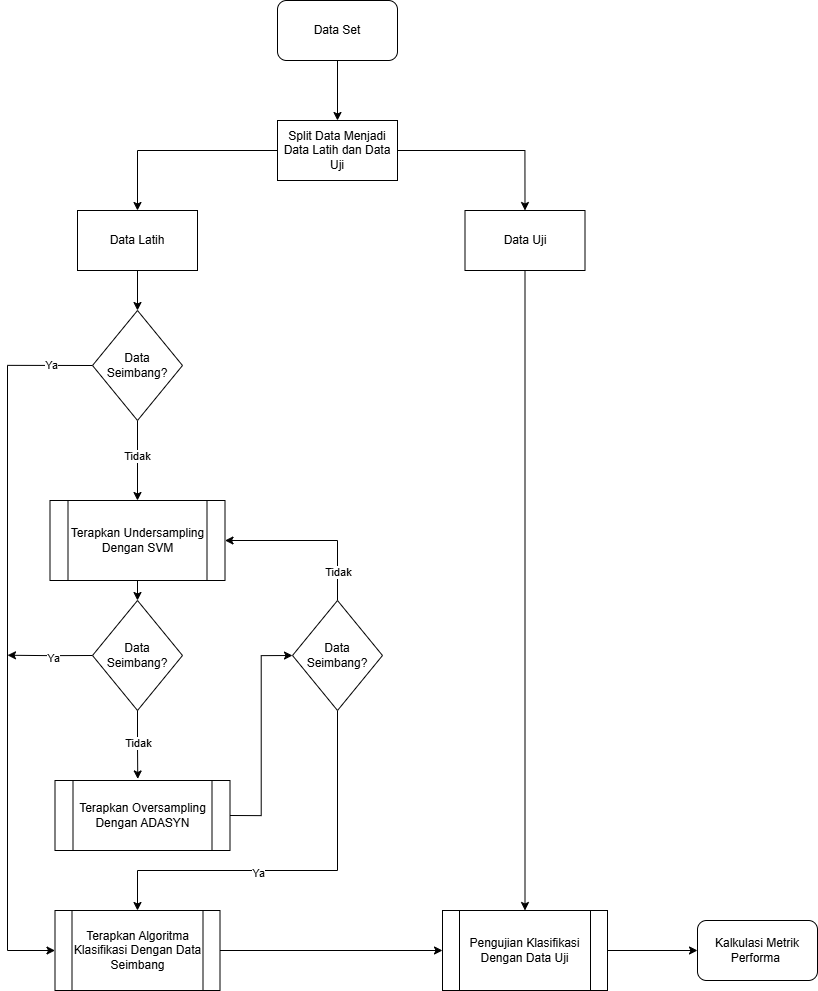
\includegraphics[width=\textwidth]{figure/HOUMFLOW.png}
    \caption{Alur Kerja Metode HOUM}
    \label{fig:2.houmflow}
\end{figure}

Alur kerja HOUM ditunjukkan pada Gambar \ref{fig:2.houmflow}. Proses kerja HOUM dimulai dengan perhitungan \textit{imbalance ratio} pada dataset untuk menentukan apakah proses penyeimbangan perlu dilakukan \cite{Eroglu2024HOUM}. Apabila distribusi kelas belum mencapai keseimbangan yang ditentukan, algoritma menjalankan dua tahap secara bergantian dalam setiap iterasi. Pada tahap pertama, SVM dilatih menggunakan dataset yang tersedia kemudian data kelas mayoritas yang berada di luar batas \textit{margin} dihapus karena dianggap kurang informatif. Pada tahap kedua, Safe-Level SMOTE digunakan untuk menambah sampel kelas minoritas di posisi yang dianggap aman berdasarkan komposisi tetangga terdekat. Kedua tahap tersebut diulang secara iteratif hingga rasio antara kelas mayoritas dan kelas minoritas mencapai keseimbangan yang diharapkan \cite{Eroglu2024HOUM}.

Pendekatan iteratif pada HOUM memberikan keunggulan karena \textit{decision boundary} SVM diperbarui pada setiap putaran berdasarkan distribusi data terkini, sehingga pemilihan data yang dihapus menjadi semakin tepat pada iterasi berikutnya \cite{Eroglu2024HOUM}. Safe-Level SMOTE yang dijalankan pada setiap iterasi dapat menyesuaikan posisi dan jumlah sampel sintetis sesuai dengan kebutuhan distribusi terbaru. Pengujian yang dilakukan oleh Eroglu dan Pir pada delapan dataset dari UCI \textit{Machine Learning Repository} menunjukkan bahwa HOUM mampu mengungguli metode pembanding seperti SMOTE, SMOTEENN, SMOTETomek, W-SIMO, dan RusAda \cite{Eroglu2024HOUM}. Hasil eksperimen menunjukkan peningkatan yang konsisten pada metrik G-mean dan ROC-AUC, yang mengonfirmasi kemampuan HOUM dalam menyeimbangkan performa klasifikasi pada kedua kelas secara bersamaan \cite{Eroglu2024HOUM}.


\subsection{\textit{Support Vector Machine} (SVM)} \label{II.svm}
Cortes dan Vapnik (1995) pertama kali memperkenalkan SVM sebagai algoritma klasifikasi yang telah menjadi salah satu metode paling banyak digunakan dalam \textit{machine learning} karena kemampuannya dalam menangani data berdimensi tinggi dan menghasilkan \textit{decision boundary} yang optimal \cite{Cervantes2020SVM}. Ide dasar SVM yaitu mencari \textit{hyperplane} pemisah yang memaksimalkan margin antara dua kelas, dimana margin didefinisikan sebagai jarak terpendek antara \textit{hyperplane} dengan sampel data terdekat dari masing-masing kelas. \textit{Hyperplane} tersebut menjadi bidang pemisah berdimensi $n-1$ dalam ruang fitur berdimensi $n$ yang memisahkan data dari dua kelas yang berbeda. Data yang terletak paling dekat dengan \textit{hyperplane} dan menentukan posisi serta orientasinya disebut sebagai \textit{support vectors} \cite{Cervantes2020SVM, Abdullah2021SVM}. Fungsi keputusan SVM untuk klasifikasi \textit{binary} dapat dirumuskan sebagaimana ditunjukkan pada \ref{eq:2.svm}.

\begin{equationcaptioned}[eq:2.svm]{
    f(x) = \text{sign}(w \cdot x + b)
}{
    Fungsi Keputusan SVM
}
\end{equationcaptioned}

Keterangan: \\
$f(x)$ = hasil prediksi kelas \\
$w$ = vektor bobot \\
$x$ = vektor fitur masukan \\
$b$ = bias

\begin{figure}[H]
    \centering
    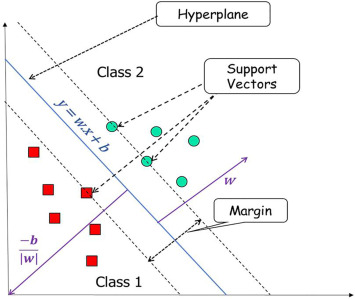
\includegraphics[width=0.6\textwidth]{figure/svm.jpg}
    \caption{Ilustrasi SVM}
    \label{fig:2.svm}
\end{figure}

Gambar \ref{fig:2.svm} merupakan ilustrasi cara kerja SVM dalam memisahkan dua kelas data. SVM mencari \textit{hyperplane} optimal yang memaksimalkan margin antara kedua kelas \cite{Cervantes2020SVM}. Margin didefinisikan sebagai jarak antara \textit{hyperplane} dengan sampel data terdekat dari masing-masing kelas, dimana sampel tersebut disebut \textit{support vectors} karena menjadi penentu posisi dan orientasi \textit{hyperplane} \cite{Abdullah2021SVM}. Vektor bobot $w$ tegak lurus terhadap \textit{hyperplane} dan menentukan arah pemisahan, sedangkan bias $b$ mengatur posisi \textit{hyperplane} terhadap titik asal. Data yang berada di sisi positif \textit{hyperplane} diklasifikasikan ke satu kelas, sedangkan data di sisi negatif diklasifikasikan ke kelas lainnya \cite{Cervantes2020SVM}. Dengan memaksimalkan margin, SVM menghasilkan model yang memiliki kemampuan generalisasi yang baik terhadap data baru yang belum pernah ditemui \cite{Cervantes2020SVM, Abdullah2021SVM}.

Pada banyak permasalahan nyata, data tidak selalu dapat dipisahkan secara linear dalam ruang fitur aslinya karena distribusi data seringkali bersifat nonlinear \cite{Cervantes2020SVM}. Untuk menangani kasus tersebut, SVM menggunakan \textit{kernel trick} yang memetakan data ke ruang fitur berdimensi lebih tinggi dimana data menjadi separabel secara linear. Fungsi kernel menghitung \textit{dot product} pada ruang berdimensi tinggi tanpa perlu melakukan transformasi secara eksplisit, sehingga komputasi tetap efisien meskipun dimensi ruang transformasi sangat besar \cite{Abdullah2021SVM, Cervantes2020SVM}. Cervantes \textit{et al.} (2020) mengidentifikasi bahwa pemilihan kernel yang tepat merupakan salah satu faktor kunci yang menentukan performa SVM pada berbagai domain aplikasi \cite{Cervantes2020SVM}. Tiga jenis kernel yang digunakan dalam penelitian ini adalah sebagai berikut:

\begin{enumerate}
    \item Kernel Linear

    Kernel linear menghitung perkalian titik antara dua vektor dengan persamaan yang ditunjukkan pada \ref{eq:2.kernel.linear}.

    \begin{equationcaptioned}[eq:2.kernel.linear]{
        K(x_i, x_j) = x_i^T x_j
    }{
        Kernel Linear
    }
    \end{equationcaptioned}

    Keterangan: \\
    $x_i$ = data latih \\
    $x_j$ = data uji

    \item Kernel Polynomial

    Kernel polynomial memiliki dua parameter utama, yaitu $c$ dan $d$, dengan persamaan yang ditunjukkan pada \ref{eq:2.kernel.poly}.

    \begin{equationcaptioned}[eq:2.kernel.poly]{
        K(x_i, x_j) = (\gamma (x_i \cdot x_j) + c)^d
    }{
        Kernel Polynomial
    }
    \end{equationcaptioned}

    Keterangan: \\
    $x_i$ = data latih \\
    $x_j$ = data uji \\
    $c$ = nilai konstan \\
    $d$ = derajat polynomial

    \item Kernel RBF (\textit{Radial Basis Function})

    Kernel RBF sering digunakan untuk data yang tidak bisa dipisahkan secara linear, dengan persamaan yang ditunjukkan pada \ref{eq:2.kernel.rbf}.

    \begin{equationcaptioned}[eq:2.kernel.rbf]{
        K(x_i, x_j) = \exp(-\gamma \|x_i - x_j\|^2)
    }{
        Kernel RBF
    }
    \end{equationcaptioned}

    Keterangan: \\
    $x_i$ = data latih \\
    $x_j$ = data uji \\
    $\|x_i - x_j\|^2$ = jarak euclidean kuadrat \\
    $\gamma$ = parameter yang menentukan pengaruh setiap sampel data latih
\end{enumerate}

\begin{figure}[H]
    \centering
    \begin{subfigure}[b]{0.4\textwidth}
        \centering
        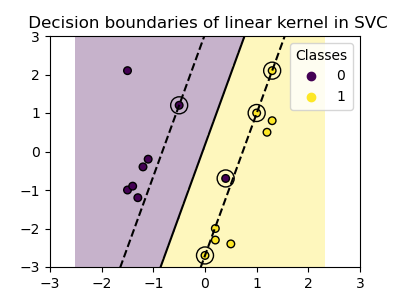
\includegraphics[width=\textwidth]{figure/linearkernel.png}
        \caption{Kernel Linear}
    \end{subfigure}
    \hspace{0.05\textwidth}
    \begin{subfigure}[b]{0.4\textwidth}
        \centering
        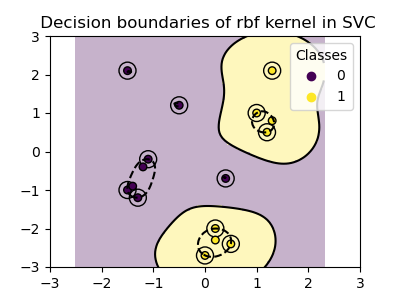
\includegraphics[width=\textwidth]{figure/rbfkernel.png}
        \caption{Kernel RBF}
    \end{subfigure}

    \vspace{0.3cm}

    \begin{subfigure}[b]{0.4\textwidth}
        \centering
        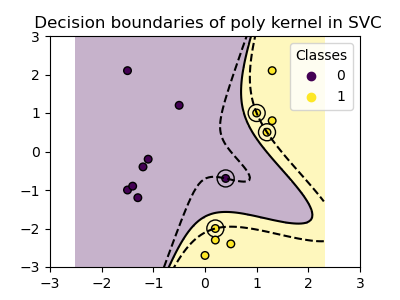
\includegraphics[width=\textwidth]{figure/polykernel.png}
        \caption{Kernel Polynomial}
    \end{subfigure}
    \caption{Ilustrasi \textit{Hyperplane} di Masing-masing Kernel \cite{ScikitLearnSVMKernels}}
    \label{fig:2.kernels}
\end{figure}

Gambar \ref{fig:2.kernels} menunjukkan visualisasi batas keputusan (\textit{decision boundary}) dari tiga kernel yang berbeda. Kernel Linear memisahkan data dengan garis lurus, kernel Polynomial menghasilkan batas keputusan melengkung, dan kernel RBF menunjukkan pola yang fleksibel sehingga cocok untuk data nonlinear.


Parameter regularisasi $C$ pada SVM berfungsi mengontrol keseimbangan antara lebar margin dan toleransi kesalahan klasifikasi pada data pelatihan, dimana nilai $C$ berada dalam rentang $0 < C < \infty$ \cite{Cervantes2020SVM}. Nilai $C$ yang kecil menghasilkan margin yang lebih lebar dan memperbolehkan lebih banyak kesalahan klasifikasi sehingga model kurang rentan terhadap \textit{overfitting}. Sebaliknya, nilai $C$ yang besar menghasilkan margin yang lebih sempit dan berusaha meminimalkan setiap kesalahan pada data pelatihan, namun berisiko \textit{overfitting} \cite{Cervantes2020SVM, Rezvani2024SVMImbalanced}. Pemilihan nilai $C$ yang tepat sangat penting karena berpengaruh langsung terhadap kemampuan generalisasi model terhadap data yang belum pernah ditemui.

SVM terbukti efektif pada data berdimensi tinggi dan telah banyak diterapkan pada berbagai domain seperti pengenalan wajah, diagnosis penyakit, analisis sentimen, dan deteksi intrusi jaringan \cite{Abdullah2021SVM}. Namun, SVM standar memiliki keterbatasan dalam menangani data tidak seimbang karena fungsi optimasinya cenderung menghasilkan \textit{hyperplane} yang bias terhadap kelas mayoritas \cite{Tang2009SVMImbalanced, Rezvani2024SVMImbalanced}. Tang \textit{et al.} (2009) mengidentifikasi bahwa pada data tidak seimbang, \textit{support vectors} lebih banyak berasal dari kelas mayoritas sehingga \textit{hyperplane} bergeser ke arah kelas minoritas \cite{Tang2009SVMImbalanced}. Rezvani \textit{et al.} (2024) mengategorikan pendekatan SVM untuk menangani data tidak seimbang ke dalam tiga kelompok, yaitu metode \textit{re-sampling}, metode algoritmik, dan metode fusi, yang masing-masing berupaya mengatasi bias melalui mekanisme yang berbeda \cite{Rezvani2024SVMImbalanced}. Berbagai modifikasi SVM untuk data tidak seimbang terus dikembangkan guna meningkatkan kemampuan algoritma ini dalam mengklasifikasikan kedua kelas secara berimbang \cite{Rezvani2024SVMImbalanced}.


\subsection{Metrik Evaluasi} \label{II.metrik}
Metrik evaluasi berfungsi sebagai ukuran kuantitatif untuk menilai seberapa baik model klasifikasi mampu melakukan prediksi terhadap data uji \cite{Sokolova2009Metrics}. Sokolova dan Lapalme (2009) menyatakan bahwa pemilihan metrik evaluasi yang tepat bergantung pada karakteristik permasalahan dan tujuan klasifikasi yang ingin dicapai \cite{Sokolova2009Metrics}. Pada domain data tidak seimbang, dibutuhkan metrik yang mampu mengukur performa model pada setiap kelas secara terpisah sehingga kemampuan model dalam mengenali kelas minoritas dapat terlihat dengan jelas \cite{Luque2019Metrics}. Fawcett (2006) menekankan bahwa teknik evaluasi berbasis kurva ROC menjadi standar untuk merangkum performa klasifikasi pada berbagai titik operasi \cite{Fawcett2006ROC}. Beberapa metrik yang umum digunakan untuk mengevaluasi performa klasifikasi pada data tidak seimbang antara lain \textit{Recall}, \textit{Precision}, G-mean, dan ROC-AUC \cite{Sokolova2009Metrics, Grandini2020Metrics}.

\subsubsection{\textit{Recall}} \label{II.recall}
\textit{Recall} atau \textit{sensitivity} mengukur proporsi sampel positif yang berhasil dideteksi oleh model dari seluruh sampel positif yang sebenarnya ada dalam dataset \cite{Luque2019Metrics}. Metrik ini sangat penting pada data tidak seimbang karena menunjukkan kemampuan model dalam mengenali kelas minoritas yang seringkali menjadi target deteksi utama. Nilai \textit{Recall} yang rendah menandakan bahwa model banyak melewatkan sampel positif yang seharusnya terdeteksi, yang disebut sebagai \textit{False Negative}. Pada kasus seperti diagnosis penyakit, nilai \textit{Recall} yang rendah bermakna banyak pasien sakit yang tidak terdiagnosis sehingga dapat berakibat fatal \cite{Fawcett2006ROC, Sokolova2009Metrics}. Rumus \textit{Recall} ditunjukkan pada \ref{eq:2.recall}.

\begin{equationcaptioned}[eq:2.recall]{
    Recall = \frac{TP}{TP + FN}
}{
    Recall (Sensitivity)
}
\end{equationcaptioned}

Keterangan: \\
$TP$ = \textit{True Positive} \\
$FN$ = \textit{False Negative}
\subsubsection{\textit{Precision}} \label{II.precision}
\textit{Precision} mengukur proporsi prediksi positif yang benar-benar termasuk sampel positif dari seluruh data yang diprediksi sebagai positif oleh model \cite{Luque2019Metrics}. Metrik ini menunjukkan seberapa akurat model ketika memberikan label positif pada suatu data, yang penting untuk menilai tingkat kepercayaan terhadap prediksi positif. Nilai \textit{Precision} yang rendah menandakan bahwa model menghasilkan banyak \textit{false alarm} atau prediksi positif yang salah sehingga mengurangi kepercayaan terhadap hasil prediksi. Pada konteks deteksi penipuan kartu kredit, nilai \textit{Precision} yang rendah berarti banyak transaksi sah yang salah ditandai sebagai penipuan dan memerlukan investigasi tambahan yang tidak perlu \cite{Sokolova2009Metrics, Grandini2020Metrics}. Rumus \textit{Precision} ditunjukkan pada \ref{eq:2.precision}.

\begin{equationcaptioned}[eq:2.precision]{
    Precision = \frac{TP}{TP + FP}
}{
    Precision
}
\end{equationcaptioned}

Keterangan: \\
$TP$ = \textit{True Positive}\\
$FP$ = \textit{False Positive}

\subsubsection{G-mean} \label{II.gmean}
G-mean atau \textit{Geometric Mean} mengukur keseimbangan performa model pada kedua kelas secara bersamaan melalui perhitungan rata-rata geometris antara \textit{sensitivity} dan \textit{specificity} \cite{Luque2019Metrics}. Metrik ini dihitung sebagai akar kuadrat dari perkalian \textit{sensitivity} yang mengukur kemampuan mendeteksi kelas positif dengan \textit{specificity} yang mengukur kemampuan mendeteksi kelas negatif. Luque \textit{et al.} (2019) membuktikan secara analitis bahwa G-mean memiliki bias bernilai nol terhadap ketidakseimbangan kelas (\textit{null-biased}), yang berarti nilai metrik ini tidak terpengaruh oleh proporsi kelas dalam dataset \cite{Luque2019Metrics}. Apabila model hanya unggul pada satu kelas namun buruk pada kelas lainnya, nilai G-mean akan turun secara signifikan karena sifat perkalian pada rata-rata geometris. Karakteristik ini menjadikan G-mean sangat cocok untuk mengevaluasi model pada data tidak seimbang, dimana keseimbangan performa pada kedua kelas merupakan tujuan utama \cite{Luque2019Metrics}. Rumus G-mean ditunjukkan pada \ref{eq:2.gmean}.

\begin{equationcaptioned}[eq:2.gmean]{
    G\text{-}mean = \sqrt{\frac{TP}{TP+FN} \times \frac{TN}{TN+FP}}
}{
    G-mean (Geometric Mean)
}
\end{equationcaptioned}

Keterangan: \\
$TP$ = \textit{True Positive}\\
$TN$ = \textit{True Negative}\\
$FP$ = \textit{False Positive}\\
$FN$ = \textit{False Negative}

Nilai G-mean yang tinggi menandakan bahwa model memiliki performa yang baik dan seimbang pada kedua kelas, yaitu kelas positif maupun kelas negatif. Metrik ini akan bernilai nol apabila model gagal total pada salah satu kelas, meskipun performa pada kelas lainnya mencapai nilai sempurna. Sifat ini sangat berguna dalam konteks data tidak seimbang dimana model yang hanya mampu mengklasifikasikan kelas mayoritas dengan benar akan tetap memperoleh G-mean senilai nol \cite{Luque2019Metrics}. Chicco dan Jurman (2023) merekomendasikan penggunaan metrik yang sensitif terhadap kedua kelas seperti G-mean dan MCC untuk menghindari kesalahan interpretasi yang sering terjadi saat menggunakan akurasi pada data tidak seimbang \cite{Chicco2023MCC}. Karakteristik tersebut menjadikan G-mean sebagai salah satu metrik yang paling sesuai untuk mengevaluasi performa model pada dataset dengan distribusi kelas yang tidak seimbang \cite{Luque2019Metrics}.

\subsubsection{ROC-AUC} \label{II.rocauc}
ROC-AUC (\textit{Receiver Operating Characteristic - Area Under the Curve}) mengukur kemampuan diskriminatif model dalam membedakan kelas positif dan kelas negatif pada berbagai nilai \textit{threshold} keputusan \cite{Fawcett2006ROC}. Kurva ROC dibentuk dengan membuat plot \textit{True Positive Rate} (TPR) terhadap \textit{False Positive Rate} (FPR) untuk setiap kemungkinan nilai ambang batas, sehingga memberikan gambaran menyeluruh tentang performa model pada seluruh titik operasi. Model dengan kemampuan diskriminatif yang baik memiliki kurva ROC yang mendekati sudut kiri atas grafik, sedangkan model yang melakukan prediksi secara acak menghasilkan garis diagonal \cite{Fawcett2006ROC}. AUC merangkum informasi dari seluruh kurva ROC ke dalam satu nilai skalar antara 0 dan 1 yang mudah dibandingkan antar model. Luque \textit{et al.} (2019) menunjukkan bahwa AUC ekuivalen dengan \textit{Bookmaker Informedness} yang ternormalisasi (\textit{BMn}) pada kasus klasifikasi dengan \textit{threshold} tunggal, sehingga AUC bersifat \textit{null-biased} terhadap ketidakseimbangan kelas \cite{Luque2019Metrics}. Rumus TPR dan FPR ditunjukkan pada \ref{eq:2.tprfpr}.

\begin{equationcaptioned}[eq:2.tprfpr]{
    TPR = \frac{TP}{TP + FN}, \quad FPR = \frac{FP}{FP + TN}
}{
    True Positive Rate dan False Positive Rate
}
\end{equationcaptioned}

Keterangan: \\
$TPR$ = \textit{True Positive Rate} \\
$FPR$ = \textit{False Positive Rate}
\begin{figure}[H]
    \centering
    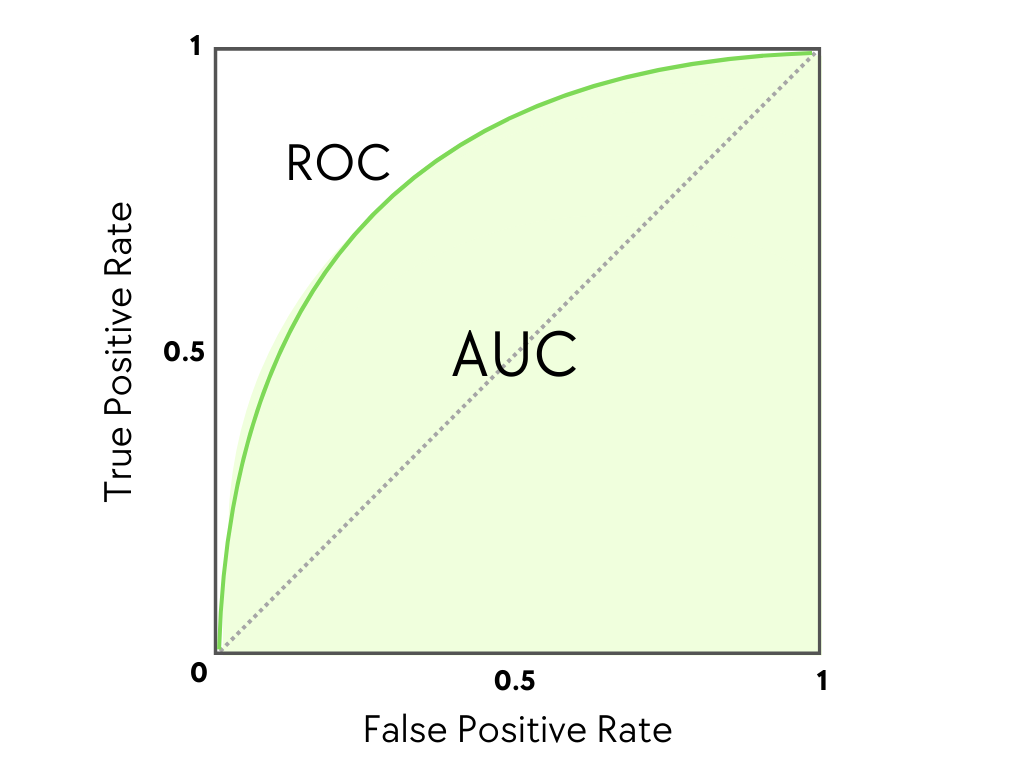
\includegraphics[width=0.9\textwidth]{figure/rocauc.png}
    \caption{Ilustrasi Kurva ROC-AUC}
    \label{fig:2.rocauc}
\end{figure}

Ilustrasi kurva ROC-AUC ditunjukkan pada Gambar \ref{fig:2.rocauc}. Nilai AUC berkisar antara 0 hingga 1, dimana nilai 1 menunjukkan model yang memiliki kemampuan diskriminatif sempurna dan nilai 0,5 menunjukkan model yang tidak lebih baik dari prediksi acak \cite{Fawcett2006ROC}. Fawcett (2006) menjelaskan bahwa AUC dapat diinterpretasikan sebagai probabilitas bahwa model memberikan skor lebih tinggi pada sampel positif yang dipilih secara acak dibandingkan sampel negatif yang dipilih secara acak \cite{Fawcett2006ROC}. Keunggulan utama ROC-AUC sebagai metrik evaluasi adalah kemampuannya untuk memberikan penilaian performa yang tidak terpengaruh oleh ketidakseimbangan distribusi kelas maupun distribusi skor keputusan \cite{Luque2019Metrics}. ROC-AUC direkomendasikan sebagai metrik standar untuk perbandingan performa model klasifikasi pada berbagai domain yang melibatkan data tidak seimbang \cite{Fawcett2006ROC, Grandini2020Metrics}. Metrik ini banyak digunakan bersamaan dengan G-mean, \textit{Recall}, dan \textit{Precision} untuk memberikan evaluasi performa yang menyeluruh pada berbagai sudut pandang \cite{Sokolova2009Metrics}.
